\section{상위 VLM 조종기}
\label{sec:upper}

\begin{figure*}[t]
\centering
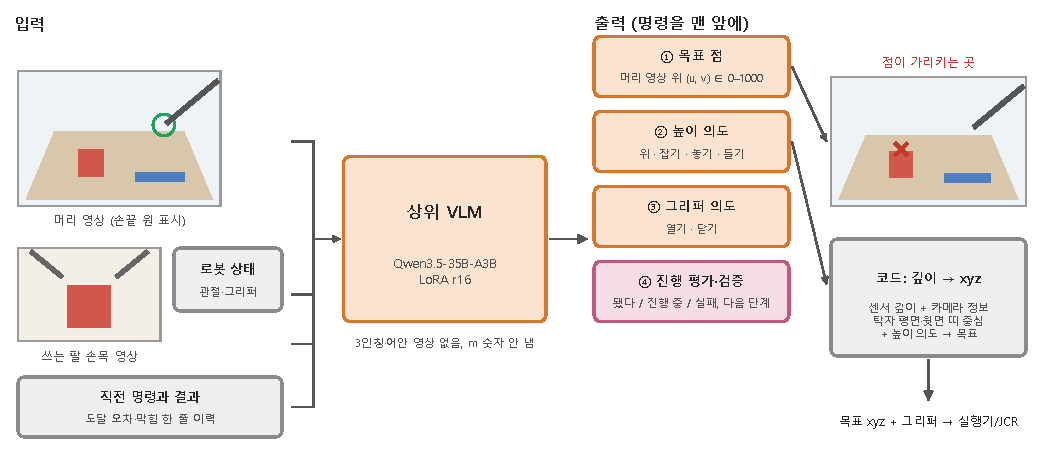
\includegraphics[width=\linewidth]{figures/f2_upper_call.pdf}
\caption{\textbf{상위 VLM 조종 한 호출.} 입력은 손끝 원만 그린 머리 영상, 표시 없는 쓰는 팔 손목 영상, 로봇 상태, 직전 명령과 결과다. 출력은 머리 영상 위 목표 점, 높이 의도, 그리퍼 의도, 진행 평가·검증이며 명령 부분을 답의 맨 앞에 둔다. 모델은 m 숫자를 말하지 않는다. 점이 가리키는 곳의 xyz는 코드가 센서 깊이와 카메라 정보로 계산한다.}
\label{fig:upper}
\end{figure*}

\subsection{입력과 출력}
\paragraph{입력.} 머리 영상(손끝 위치를 알리는 원만 그림)과 지금 쓰는 팔의 손목 영상(아무것도 그리지 않음), 로봇 자기 상태(관절, 그리퍼 폭), 직전 명령과 그 결과(도달 오차·막힘을 적은 한 줄 이력)다(\cref{fig:upper}). 3인칭·어안 영상은 정확도 위험이 있어 쓰지 않는다. 영상에 격자는 그리지 않는다. 로봇 자기 정보(좌표계, 그리퍼 형상, 카메라 자세·내부값)는 URDF·관절 상태·camera\_info에서 코드가 만든다.

\paragraph{출력: 줄기 D.} 모델은 (i) 머리 영상 위의 목표 점(0--1000 정규화), (ii) 높이 의도(위, 잡기, 놓기, 들기), (iii) 그리퍼 의도, (iv) 진행 평가·검증을 낸다. 목표 xyz는 코드가 계산한다. 센서 깊이와 카메라 정보로 탁자 평면을 맞추고, 평면 위 물체 영역의 윗면 띠 중심을 잡은 뒤 높이 의도에 맞춰 목표를 정한다. 실물에서는 머리 스테레오와 손목 D405의 깊이가 필요하며, 이는 사람이 준 정보가 아니라 측정값이다.

\subsection{왜 D인가}
거리를 m 숫자로 직접 내는 줄기는 본 적 없는 탁자 높이에서 무너졌다. 한 높이 데이터로 학습한 8B와 35B 모두 새 높이 3D 오차가 \tentative{약 31\,mm}였고, 대부분 z 오차였다. 모델 크기로 풀리지 않는다. 같은 편을 출력 형식만 바꿔 비교하자 깊이 점만 새 높이에서 \tentative{3.5--3.6\,mm}를 유지했다(깊이 없는 xyz \tentative{31--71\,mm}, 폐루프 \tentative{8/8}). 깊이가 있으면 쓰고 없으면 xyz를 직접 내는 하이브리드 H와의 비교에서도 D가 새 물체에서 \tentative{4.0} 대 \tentative{83.7\,mm}로 이겼다(\cref{sec:evidence}).

사람이 준 손 정보(탁자 높이 등)는 넣지 않는다. 참 탁자 높이를 입력으로 받은 판만 새 높이에 맞았고(\tentative{4.0\,mm}), 학습 때만 그 정보를 쓰는 세 방법은 \tentative{10.9--20.5\,mm}였다. 영상 하나로는 탁자 높이를 약 2\,cm보다 정확히 알 수 없고, 실제 환경에는 참값이 없다. 척도와 높이는 깊이가 맡는다.

\subsection{판단의 역할}
상위는 명령만 내지 않고 매 답에 판단을 싣는다.
\begin{itemize}
  \item \textbf{진행 평가:} 끝낸 일·지금 하는 일·남은 일과 현재 단계의 상태(됐다 / 진행 중 / 실패).
  \item \textbf{실패 감지와 다시 계획:} 직전 명령의 결과(측정 이력, VLA 이상 신호, 새 영상)가 의도와 어긋나면 실패로 판정하고 목표를 다시 낸다.
  \item \textbf{다음 단계 선택:} 결과를 확인한 뒤 잡기·나르기·놓기 가운데 다음을 고른다. 쥠·놓음의 확정 근거는 T1이다.
\end{itemize}
판단 정확도(진행 판정의 정밀도·재현율, 실패 감지까지의 지연)를 재는 평가 세트는 아직 없다. 이 지표는 \cref{sec:questions}의 첫 질문이다. 실패 인지·재시도를 위한 회복 데이터도 이번 본 학습에는 넣지 않았다.

\subsection{학습}
\label{sec:upper_train}
라벨은 시뮬 참값(특권 정보로 계산)이다. 로봇 기하와 시뮬 상태에서 도출한 규칙이 같은 요청에 대해 낸 답을 정답으로 쓴다. 공개 로봇 데이터는 행동 라벨이 아니라 머리 시점 영상 위의 점 라벨(대상, 놓을 곳, 그리퍼)로만 쓴다~\cite{molmoact2026}. 공개/시뮬 비율은 $\min(0.75,\ 2\times\text{공개 풀}/\text{시뮬 행})$이고 같은 행의 반복은 2배까지다.

\paragraph{본 35B.} Qwen3.5-35B-A3B에 LoRA(r16, $\alpha$32, 어텐션·DeltaNet·공유 전문가), lr $10^{-4}$, H200 4장 전역 배치 24로 3 에폭(약 25,300걸음) 학습한다. 데이터는 202,397행이다(L8S 139,603행 + 공개 점 62,794행, \cref{sec:data}). 2026-09-30 15:57 KST에 시작했고 \tentative{10/1 오후} 끝날 예정이다. 최적 에폭은 학습에 쓰지 않은 L8S 보류 검증 분할(편 단위 3\,\%)의 20\,mm 초과 실패율로 고르며, OOD·새 물체 세트로는 고르지 않는다. 이 규칙은 결과 전에 사전 등록했다.

\paragraph{다음.} 도착 전에 다음 명령을 내는 행(\cref{sec:mesh})과 L9 데이터(\cref{sec:data})를 넣은 다음 본 학습은 기본 모델부터 섞어 한 번에 학습한다.
